% Part: sets-functions-relations
% Chapter: infinite
% Section: hilberts-hotel
%
\documentclass[../../../include/open-logic-section]{subfiles}

\begin{document}

\olfileid[fr]{sfr}{infinite}{hilbert}
\olsection{L'hôtel de Hilbert}

L'ensemble des entiers naturels est manifestement infini. Aussi, si nous
ne voulons pas \emph{supposer d'emblée l'existence} des entiers naturels,
notre première étape doit consister à caractériser un ensemble infini
dans des termes qui ne nécessitent pas de mentionner les entiers naturels
eux-mêmes. Voici une approche intéressante, présentée par Hilbert dans
ses cours de l'hiver 1924--1925.\footnote{Note de l'édition française :
la source indique 1924. Nous précisons ici l'intervalle du semestre
d'hiver 1924--1925 donné par les éditeurs pour ces cours, sans attribuer
une date précise à cette séance.} Il nous demande d'imaginer
\begin{quote}
[\ldots] un hôtel ayant un nombre fini de chambres. Toutes ces chambres
doivent être occupées par exactement un client. Si les clients échangent
maintenant leurs chambres d'une manière quelconque, [mais] de telle sorte
que chaque chambre contienne encore au plus une personne, aucune chambre
ne se libérera, et le propriétaire de l'hôtel ne pourra pas créer ainsi
une place pour un client qui vient d'arriver [\ldots
\textparagraph \ldots]

Supposons maintenant que l'hôtel possède une infinité de chambres
numérotées $1$, $2$, $3$, $4$, $5$, \dots, chacune occupée par exactement
un client. Dès qu'un nouveau client arrive, il suffit au propriétaire
de déplacer chacun des clients déjà présents dans la chambre dont le
numéro est supérieur d'une unité, et la chambre~$1$ sera libre pour le
client qui vient d'arriver.
	\begin{center}
		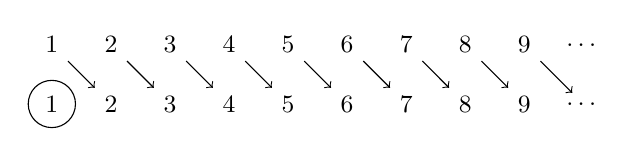
\begin{tikzpicture}[scale = .75]
		\foreach \x in {1, 2, 3, 4, 5, 6, 7, 8, 9}
		{
			\node (\x a) at (\x, 1) {\small{\x}};
			\node (\x b) at (\x, 2) {\small{\x}};
		}
		\node (dotsa) at (10, 1) {\small{\ldots}};
		\node (dotsb) at (10, 2) {\small{\ldots}};
		\draw[->] (1b)--(2a);
		\draw[->] (2b)--(3a);
		\draw[->] (3b)--(4a);
		\draw[->] (4b)--(5a);
		\draw[->] (5b)--(6a);
		\draw[->] (6b)--(7a);
		\draw[->] (7b)--(8a);
		\draw[->] (8b)--(9a);
		\draw[->] (9b)--(dotsa);
		\draw (1,1) circle (.4);
		\end{tikzpicture}
	\end{center}
	(publié dans \citealt[730]{EwaldSieg2013} ; traduction française
	d'après la traduction anglaise donnée dans la source)
\end{quote}
Le point crucial est que l'hôtel de Hilbert possède une infinité de
chambres ; nous pouvons prendre cette explication pour définir ce que
cela signifie. C'était précisément l'approche de Dedekind, présentée
ici, bien entendu, au prix d'un anachronisme considérable : sa définition
date de \citeyear{Dedekind1888}.

\begin{defn}\ollabel{defn:DedekindInfinite}
Un ensemble $A$ est \emph{infini au sens de Dedekind} si et seulement
s'il existe !!a{injection} de~$A$ dans une partie propre de~$A$.
Autrement dit, il existe un élément $o \in A$ et !!a{injection}
$f \colon A \to A$ tels que $o \notin \ran{f}$.
\end{defn}

\end{document}
